\section{有限温度的时间格林函数}

\subsection{推广的莱曼表示}

首先拷贝热力学格林函数的定义, $t_1 > t_2$时,

\begin{eqnarray*}
% \nonumber to remove numbering (before each equation)
  iG_{\alpha \beta} (x_1 t_1, x_2 t_2) &=& Tr \left\{ e^{\beta \Omega}
e^{-\beta K } \psi_\alpha (x_1 t_1) \psi_\beta^\dagger (x_2
t_2) \right\} \\
  {} &=& \left\langle \psi_\alpha (x_1 t_1)
\psi_\beta^\dagger (x_2 t_2) \right\rangle
\end{eqnarray*}

其中, $K = H - \mu N$

\begin{eqnarray*}
% \nonumber to remove numbering (before each equation)
  \psi_\alpha(x_1 t_1) &=& e^{iK t_1} e^{-i P x_1} \psi_\alpha e^{i P x_1} e^{-i K t_1 } \\
  \psi^{\dagger}_{\beta} (x_2 t_2) &=& e^{i K t_2} e^{-i P x_2} \psi^{\dagger}_{\beta} e^{i P x_2} e^{-i K t_2 }
\end{eqnarray*}


假设系统是空间均匀的, $P$, $H$, $N$两两对易, 有共同本征态,
记作$\left| n \right\rangle$, 本征值分别为$P_n$, $E_n$, 和$N_n$ (或
$K_n = E_n - \mu N_n$).

求Trace运算就是$\sum_n \left\langle n \right| \rho A \left| n
\right\rangle $,

\begin{equation*}
iG(1,2) = \sum_{nm} \left\langle n \right| \rho \psi(1) \left| m
\right\rangle \left\langle m \right| \psi^\dagger(2) \left| n
\right\rangle
\end{equation*}

这里,

\begin{eqnarray*}
% \nonumber to remove numbering (before each equation)
  \left\langle n \right| \rho \psi(1) \left| m \right\rangle &=& e^{\beta \Omega} e^{-\beta K_n} e^{i K_n t_1} e^{-i P_n x_1}
e^{i P_m x_1} e^{- i K_m t_1}  \left\langle n \right| \psi_\alpha
\left| m \right\rangle \\
  {} &=& e^{\beta \Omega} e^{-\beta K_n} e^{- i(K_m - K_n) t_1} e^{i (P_m
- P_n) x_1} \left\langle n \right| \psi_\alpha \left| m
\right\rangle
\end{eqnarray*}

类似地,

\begin{eqnarray*}
% \nonumber to remove numbering (before each equation)
  \left\langle m \right| \psi^\dagger(2) \left| n \right\rangle &=& e^{iK_m t_2} e^{-i P_m x_2} e^{i P_n x_2} e^{-i K_n t_2}
\left\langle m \right| \psi_\beta^\dagger \left| n \right\rangle \\
  {} &=& e^{i(K_m - K_n) t_2} e^{-i (P_m - P_n) x_2 } \left\langle m
\right| \psi_\beta^\dagger \left| n \right\rangle
\end{eqnarray*}


令:

\begin{eqnarray*}
% \nonumber to remove numbering (before each equation)
  P_{mn} &=& P_m - P_n \\
  \omega_{mn} &=& K_m - K_n
\end{eqnarray*}


$iG(1,2)$, $t_1 > t_2$可表示为:


\begin{equation*}
iG(1,2) = e^{\beta \Omega} \sum_{nm} e^{-\beta K_n} e^{iP_{mn}(x_1 -
x_2)} e^{-i\omega_{mn} (t_1 - t_2)} \left\langle n \right|
\psi_\alpha \left| m \right\rangle \left\langle m \right|
\psi_\beta^\dagger \left| n \right\rangle
\end{equation*}

对$t_1 < t_2 $, 需要计算$Tr \left\{ \rho \psi_2^\dagger \psi_1
\right\} = \sum_{nm} \left\langle n \right| \rho \psi_2^\dagger
\left| m \right\rangle \left\langle m \right| \psi_1 \left| n
\right\rangle $, 与$t_1 > t_2$的展开比较, $Tr \left\{ \rho \psi_1
\psi_2^\dagger \right\} = \sum_{nm} \left\langle n \right| \rho
\psi_1 \left| m \right\rangle \left\langle m \right| \psi_2^\dagger
\left| n \right\rangle $. 对$t_1 < t_2$, 将求和指标$n,m$互换, 得到:

\begin{equation*}
Tr \left\{ \rho \psi_2^\dagger \psi_1 \right\} = \sum_{nm}
\left\langle m \right| \rho \psi_2^\dagger \left| n \right\rangle
\left\langle n \right| \psi_1 \left| m \right\rangle
\end{equation*}

由上式, 我们可直接写出$t_1 < t_2$时的$iG(1,2)$,


\begin{equation*}
iG(1,2) = \mp e^{\beta \Omega} \sum_{nm} e^{-\beta K_m}
e^{iP_{mn}(x_1 - x_2)} e^{-i \omega_{mn}(t_1 - t_2)} \left\langle n
\right| \psi_\alpha \left| m \right\rangle \left\langle m \right|
\psi_\beta^\dagger \left| n \right\rangle
\end{equation*}

现在令, $x=x_1 - x_2$, $t=t_1 - t_2$, 得到$iG_{\alpha
\beta}(xt)$的表达式, 让后将其变换到动量, 频率空间$iG_{\alpha
\beta}(p, \omega)$.

FT的定义式为:


\begin{equation*}
G(p, \omega) = \int d^3x dt e^{-ipx}e^{i \omega t} G(xt)
\end{equation*}


这里对$t$的积分, 会因$t>0$, $t<0$分成两部分,
利用如下积分关系\footnote{利用关系: $\frac{1}{\omega \pm i \eta } =
P \frac{1}{\omega} \mp i \pi \delta(\omega ) $}:

\begin{eqnarray*}
% \nonumber to remove numbering (before each equation)
  \int_0^{\infty} dt e^{i \omega t} &=& \frac{i}{\omega + i \eta} = \frac{i}{\omega} + \pi \delta(\omega) \\
  \int_{-\infty}^0 dt e^{i \omega t} &=& - \frac{i}{\omega - i \eta}
  = - \frac{i}{\omega} + \pi \delta (\omega)
\end{eqnarray*}

对$x$的积分, 需要用到关系:

\begin{equation*}
\delta(  \vec p- \vec P_{mn}) =\frac{1}{(2\pi)^3} \int d^3 x e^{-i
(\vec p - \vec P_{mn})\cdot \vec x}
\end{equation*}

求得,


\begin{eqnarray*}
% \nonumber to remove numbering (before each equation)
  G_{\alpha \beta} (p, \omega) &=& (2\pi)^3 e^{\beta \Omega} \sum_{nm}
\left\langle n \right| \psi_\alpha \left| m \right\rangle
\left\langle m \right| \psi_\beta^\dagger \left| n \right\rangle
\delta(p-P_{mn})  \\
{} & \times &   \left\{ \frac{e^{-\beta K_n}}{\omega - \omega_{mn} +
i \eta} \pm \frac{e^{-\beta K_m}}{\omega - \omega_{mn} - i \eta}
\right\}
\end{eqnarray*}

假设哈密顿量中不含自旋指标, 如$H = \left( {\begin{array}{*{20}c}
   {H{}_{ +  + }} & 0  \\
   0 & {H_{ -  - } }  \\
 \end{array} } \right)$, $H_{++} = H_{--}$, $G_{\alpha \beta}(p, \omega) = \delta_{\alpha \beta} G(p,
 \omega)$, 于是:

 \begin{equation*}
 G(p,\omega) = \frac{1}{2S+1} G_{\alpha \alpha} (p, \omega)
 \end{equation*}

这里的$G_{\alpha \alpha}$要对自旋指标$\alpha$求和,

\begin{eqnarray*}
% \nonumber to remove numbering (before each equation)
G_{\alpha \alpha} (p, \omega) &=& (2\pi)^3 e^{\beta \Omega} \sum_{nm,\alpha} | \left\langle n \right| \psi_\alpha \left| m \right\rangle  |^2 \delta(p-P_{mn}) e^{-\beta K_n}    \\
  {} & \times & \left\{ P \frac{1}{\omega - \omega_{mn}} [1 \pm e^{-\beta \omega_{mn}}] - i \pi \delta(\omega - \omega_{mn}) [1 \mp e^{-\beta \omega_{mn}}] \right\}
\end{eqnarray*}

现在来讨论格林函数$G(p, \omega)$虚部与实部之间的关系,

首先$\omega_{mn} \to \omega'$,

\begin{eqnarray*}
% \nonumber to remove numbering (before each equation)
  G(p, \omega) &=& \sum_{nm, \alpha} ... \\
  {} &=& \int d \omega' ...\left\{ P
\frac{1}{\omega - \omega'} [1 \pm e^{-\beta \omega'}] - i \pi
\delta(\omega - \omega') [1 \mp e^{-\beta \omega'}] \right\}
\end{eqnarray*}

由上式, 可推出关系:

\begin{equation*}
Re G(p, \omega) = \frac{P}{\pi} \int_{-\infty}^{\infty} d\omega'
\left[ \tanh \frac{\beta \omega'}{2} \right]^{\mp 1} \frac{Im G(p,
\omega')}{\omega' - \omega}
\end{equation*}


``$-$''对应费米子, ``$+$''对应玻色子。

现在引入超前和推迟热力学格林函数, $G^R$, $G^A$,
分别在上下半平面得到解析函数,

\begin{eqnarray*}
% \nonumber to remove numbering (before each equation)
iG^R(1,2) &=& \theta(t_1 - t_2) Tr \left\{ \rho [\psi(1), \psi^\dagger(2)]_{\pm} \right\} \\
iG^A(1,2) &=& - \theta(t_2 - t_2) Tr \left\{ \rho [\psi(1),
\psi^\dagger(2)]_{\pm} \right\}
\end{eqnarray*}

变换到动量, 频率空间,

\begin{eqnarray*}
% \nonumber to remove numbering (before each equation)
G^R (p, \omega) &=& \frac{(2\pi)^3}{2S+1} e^{\beta
\Omega}\sum_{nm,\alpha} e^{-\beta (E_n - \mu N_n)}
\left|\psi_{nm,\alpha} \right|^2 \delta(p-P_{mn}) \\
{} & \times & \left\{ \frac{1}{\omega - \omega_{mn}} -i \pi \delta(\omega -\omega_{mn}) (1 \pm e^{-\beta \omega_{mn}}) \right\}  \\
G^A(p, \omega) &=& \frac{(2\pi)^3}{2S+1} e^{\beta
\Omega}\sum_{nm,\alpha} e^{-\beta (E_n - \mu N_n)}
\left|\psi_{nm,\alpha} \right|^2 \delta(p-P_{mn}) \\
{} & \times &  \left\{ \frac{1}{\omega - \omega_{mn}} + i \pi
\delta(\omega -\omega_{mn}) (1 \pm e^{-\beta \omega_{mn}}) \right\}
\end{eqnarray*}


可证明,

\begin{equation*}
Re G^{R,A}(p, \omega) = \frac{P}{\pi} \int_{-\infty}^{\infty}
d\omega' \frac{Im G^{R,A} (p, \omega')}{ \omega' - \omega}
\end{equation*}

通过恰当地定义谱函数$\rho(p, \omega) = \sum_{nm,\alpha}...$,
我们把$G^{R,A}$改写为:

\begin{eqnarray*}
% \nonumber to remove numbering (before each equation)
  G^R (p, \omega) &=& \int_{-\infty}^{\infty} \frac{d\omega'}{2 \pi} \frac{\rho(p, \omega')}{\omega - \omega' + i\eta } \\
  G^A (p, \omega) &=& \int_{-\infty}^{\infty} \frac{d\omega'}{2 \pi} \frac{\rho(p, \omega')}{\omega - \omega' - i\eta }
\end{eqnarray*}

可见$G^{R,A}$分别在上、下半平面解析。


\subsection{求和规则}

我们可以证明, 对态密度$\rho(p, \omega)$, 满足如下求和规则(sum rule):

\begin{equation}\label{sum rule}
\int_{-\infty}^{\infty} \frac{d \omega}{2 \pi} \rho(p, \omega) = 1
\end{equation}

证:首先构造如下积分,

\begin{equation*}
I = \int_{-\infty}^{\infty} \frac{d \omega}{2 \pi} i G^R(p, \omega)
e^{-i \omega \eta} = i \int_{-\infty}^{\infty}
\int_{-\infty}^{\infty} \frac{d \omega d \omega'}{(2\pi)^2}
\frac{\rho(p, \omega') e^{-i\omega \eta}}{\omega - \omega' + i \eta}
\end{equation*}

我们先计算上式中对$d \omega$的积分, 这里需构造积分回路如图(\ref{sum
rule contour}).

\begin{equation*}
i \int_{-\infty}^{\infty}\frac{d\omega}{2\pi}\frac{e^{-i \omega
\eta}}{\omega - \omega' + i \eta} =1
\end{equation*}

\begin{figure}[h]
\begin{center}
  % Requires \usepackage{graphicx}
  \includegraphics[width=6cm]{Finite/sum-rule-contour.ps}\\
  \caption{$e^{-i \omega \eta}$保证通过下半平面大圆的积分为零.}\label{sum rule contour}
\end{center}
\end{figure}

现在留下的就只是对$d\omega'$的积分,

\begin{equation*}
I = \int_{-\infty}^{\infty} \frac{d \omega'}{2 \pi} \rho (p,
\omega') = \int_{-\infty}^{\infty}\frac{d \omega}{2 \pi} i G^R (p,
\omega) e^{-i \omega \eta}
\end{equation*}

考虑上式中对$d \omega$ 的积分,

\begin{equation*}
I = \int_{-\infty}^{\infty}\frac{d \omega}{2 \pi} i G^R (p, \omega)
e^{-i \omega \eta} = i G^R(p, \eta)=  \int d^3 x e^{-i px} i G^R (x,
\eta)
\end{equation*}

上式中的$iG^R(x, \eta)$是,

\begin{equation*}
i G^R (x, \eta) = \frac{i}{2S+1} \sum_{\alpha} G_{\alpha
\alpha}^R(x, \eta) = \frac{1}{2S+1} Tr \left\{\rho_G [\psi_\alpha
(x, \eta), \psi_\alpha^\dagger (0,0)]_{\pm} \right\}
\end{equation*}

由于$\eta \to 0^+$, $\psi_\alpha(x,\eta) \to \psi_\alpha(x,0)$,
现在, 上式中的求迹运算为,

\begin{equation*}
Tr \left\{\rho_G [\psi_\alpha (x), \psi_\alpha^\dagger (0)]_{\pm}
\right\} = e^{\beta \Omega} \sum_{n, \alpha} e^{-\beta K_n}
\left\langle n \right| [\psi_\alpha (x), \psi_\alpha^\dagger
(0)]_{\pm} \left| n \right\rangle
\end{equation*}

场算符$\psi, \psi^\dagger$ 满足:

\begin{equation*}
[\psi_\alpha (x), \psi_\alpha^\dagger (0)]_{\pm} = \delta_{\alpha
\alpha} \delta (x)
\end{equation*}

因此,

\begin{equation*}
iG^R (x, \eta) =\frac{1}{2S+1} \sum_\alpha \left\{ \delta_{\alpha
\alpha} \delta(x) \right\} = \delta (x)
\end{equation*}

因此,

\begin{eqnarray*}
% \nonumber to remove numbering (before each equation)
  I &=& \int_{-\infty}^{\infty} \frac{d \omega}{2 \pi} \rho(p, \omega) \\
  & = & \int d^3 x e^{-i px} i G^R (x, \eta) = \int d^3 x e^{-i px} \delta(x) = 1
\end{eqnarray*}

\subsection{松原函数和解析延拓}

松原函数的定义是:

\begin{equation}
\mathcal{G} (x, \tau) = -\frac{1}{2s+1} Tr \{ e^{\beta \Omega} e^{- \beta K } \psi_{\alpha} (x,\tau) \psi_{\alpha}^\dagger (0)  \}  
\end{equation}

这里:$\psi_{\alpha}(x,\tau) = e^{-i P x } e^{K \tau} \psi_{\alpha}  e^{- K \tau} e^{i P x} $

类似先前的推导:

\begin{equation}
\mathcal{G}(x,\tau) = -\frac{ e^{\beta \Omega} }{2s+1} \sum\limits_{nm} e^{ - \beta K_n} e^{i P_{mn} x - \omega_{mn} \tau} \left| \left\langle n \right|  \psi_{\alpha} \left| m \right\rangle \right|^2 
\end{equation}

傅里叶变换,把宗量变为$p, i \omega$

\begin{eqnarray*}
\mathcal{G}(p, i \omega_l) &=& \int d^3 x \int_0^{\beta} d \tau e^{ -ipx + i \omega_l \tau } \mathcal{G} (x,\tau)    \\
{} &=& \frac{e^{\beta \Omega}}{ 2s+1 } \sum\limits_{nm} e^{-\beta K_n} (2\pi)^3 \delta(p - P_{mn}) \left| \left\langle n \right| \psi_{\alpha} \left| m \right\rangle  \right|^2 (1 \pm e^{-\beta \omega_{mn}} )\frac{1}{ i \omega_l - \omega_{mn}}
\end{eqnarray*}

这里由于$\tau$的取值是$ - \beta \to \beta$,$\omega_l$的取值是离散的,费米子位于奇数格点,而玻色子位于偶数格点。

利用谱函数$\rho (p, \omega)$的定义\footnote{蔡建华 \& 龚昌德:公式(3.6.19)},将$\mathcal{G} (p, i \omega_l )$改写为:

\begin{equation}
\mathcal{G}(p, i \omega_l) = \int_{-\infty}^{\infty} \frac{d \omega' }{2 \pi} \frac{\rho(p,\omega')}{ i \omega_l - \omega'}
\end{equation}

$\mathcal{G}(p, i \omega_l)$是个定义在分立点集$\{ i \omega_l  \}$上的复函数,我们将其延拓到整个复平面,定义复函数:

\begin{equation}
\Gamma (p, z) = \int_{-\infty}^{\infty} \frac{d \omega'}{2 \pi} \frac{\rho(p, \omega')}{z - \omega'} 
\end{equation}

$\Gamma(p,z)$与$G^R$,$G^A$,$\mathcal{G}$的关系是:

\begin{eqnarray}
G^R (p, \omega) &=& \Gamma (p, \omega + i \eta) \\
G^A (p, \omega) &=& \Gamma (p, \omega - i \eta) \\
\mathcal{G} (p, i \omega_l) &=& \Gamma (p, i \omega_l)
\end{eqnarray}

如果知道在分立点集$\{ i \omega_l \}$上的$\Gamma (p, z)$,需解析延拓到整个复$z$平面。这种解析延拓一般来说不是唯一的,假设$\Gamma (p,z)$是一个可能的延拓,对任意整数$p'$,函数$e^{2 \pi p' z / \omega_n} \Gamma(p,z) $是另一个可能的延拓。

利用求和规则(Sum Rule),当$\left| z \right| \to \infty$,$\Gamma (p, z) \to \frac{1}{z}$,我们能够挑选合适的解析延拓,并保证是唯一的\footnote{费特 \& 瓦里克:pp379;G. Baym \& N. D. Mermin,J. Math. Phys.,2:232(1961) }。

如果我们求出了$\mathcal{G}(p, i \omega_l) $,我们也就求出了$G^{R,A} (p, \omega)$

我们可以证明:

\begin{equation}
\rho(p, \omega) = i \left[ G^R (p, \omega) - G^A (p, \omega) \right]
\end{equation}

一般把$i \omega_l$形式上当作连续变量,直接从$\mathcal{G} (p, i \omega_l)$计算$\rho(p, \omega)$


\begin{equation}
\rho(p, \omega) = i \left[ \mathcal{G} (p, i \omega_l )|_{i \omega_l = \omega + i \eta}  - \mathcal{G} (p, i \omega_l )|_{i \omega_l = \omega - i \eta} \right]
\end{equation}

\subsection{态密度}

以费米子为例讨论态密度$N(\omega)$和热力学格林函数的关系。

定义:

\begin{eqnarray}
G_{\alpha \beta}^{>} (xt,x't') &=& -i Tr \{ e^{\beta (\Omega - K) }  \psi_{\alpha} (xt) \psi_{\beta}^{\dagger} (x't')   \} \\
G_{\alpha \beta}^{<} (xt,x't') &=& i Tr \{ e^{\beta ( \Omega - K) }   \psi_{\beta}^{\dagger} (x't') \psi_{\alpha} (xt)  \}
\end{eqnarray}

把场算符换到动量空间:

\begin{eqnarray}
\psi_{\alpha} (xt) &=& \frac{1}{\sqrt{V}} \sum\limits_p e^{i px} a_{p \alpha} (t) \\
\psi^{\dagger}_{\beta} (x't') &=& \frac{1}{\sqrt{V}} \sum\limits_p e^{ - i px' } a^{\dagger}_{p \beta} (t')
\end{eqnarray}

把上式代入$G_{\alpha \beta}^{>}$,$G_{\alpha \beta}^{<}$


\begin{eqnarray*}
G_{\alpha \beta}^{>} (xt,x't') &= & -\frac{i}{V} \sum\limits_{pp'} e^{ipx -ip'x'} \left\langle a_{p \alpha}(t)  a^{\dagger}_{p' \beta} (t') \right\rangle   \\
{}&=& -\frac{i}{V} \sum\limits_p e^{ip(x-x')} \left\langle a_{p \alpha}(t)  a^{\dagger}_{p \beta} (t') \right\rangle
\end{eqnarray*}

这里要利用反对易关系:$\{ a_p , a^{\dagger}_{p'}  \} = \delta (p - p') $

类似地,还有:

\begin{equation*}
G_{\alpha \beta}^{<} (xt,x't') = \frac{i }{V } \sum\limits_p e^{i p (x-x')} \left\langle a^{\dagger}_{p \beta} (t') a_{p \alpha} (t)   \right\rangle
\end{equation*}

由此可求出傅里叶变换系数$G^{>}(p,\omega)$:

\begin{eqnarray*}
G^{>}_{\alpha \beta} (p,\omega) &=& -i \int dt e^{i \omega ( t - t' )} \left\langle  a_{p \alpha}(t) a^{\dagger}_{p \beta} (t')   \right\rangle \\
{} & = & -i \int dt e^{i \omega t } \left\langle  a_{p \alpha}(t) a^{\dagger}_{p \beta} (0)   \right\rangle
\end{eqnarray*}

类似地,我们可求:

\begin{equation*}
G^{<}_{\alpha \beta} (p,\omega) = i \int dt e^{i \omega t} \left\langle a^{\dagger}_{p \beta} (0)  a_{p \alpha} (t)  \right\rangle
\end{equation*}

现在定义$N^{>} (\omega) $为由$m \to n$,使态$n$增加一个粒子而使其能量增加$\omega $可利用的空状态数。

\begin{equation}
N^{>} (\omega) = \frac{1}{V} \sum\limits_p \sum\limits_m \left| \left\langle m \right| a^{\dagger}_{p \alpha}  \left|  n  \right\rangle  \right|^2 \delta(E_m - E_n - \omega)
\end{equation}

在零温下,我们可以证明:

\begin{equation}
N^{>} (\omega) = \frac{1}{V} \sum\limits_p \int \frac{dt }{2 \pi } e^{i \omega t } \left\langle n \right|  a_{p \alpha} (t)  a^{\dagger}_{p \alpha} (0) \left| n  \right\rangle
\end{equation}

在有限温度下,对上式求统计平均:

\begin{equation}
N^{>} (\omega , T) = \frac{1}{V}  \sum\limits_p \int \frac{dt }{2 \pi } e^{i \omega t } \left\langle a_{p \alpha} (t) a^{\dagger}_{p \alpha } (0) \right\rangle
\end{equation}

$N^{>} (\omega, T)$的意义是:对一个处在热平衡态的系统,当增加一个粒子而使其能量增加$\omega $时可利用的空状态数。

类似地,我们可定义$N^{<} (\omega , T )$

\begin{equation}
N^{<} (\omega , T) = \frac{1}{V}  \sum\limits_p \int \frac{dt }{2 \pi } e^{i \omega t } \left\langle  a^{\dagger}_{p \alpha } (0)  a_{p \alpha} (t)  \right\rangle
\end{equation}

$N^{<} (\omega, T)$的意义是:对一个处在热平衡态的系统,当除去一个粒子而使其能量减少$\omega $时可利用的满状态数。($ n \to m$)

我们可以证明:

\begin{eqnarray}
N^{>} (\omega, T) &=& \frac{i}{2 \pi V } \sum\limits_p G^{>}_{\alpha \alpha} (p, \omega)  \\
N^{<} (\omega, T) &=& - \frac{i }{2 \pi V} \sum\limits_p G^{<}_{\alpha \alpha} (p, \omega) 
\end{eqnarray}

能量为$\omega $的单粒子态密度$N(\omega)$是空状态数和满状态数之和。

\begin{eqnarray*}
N(\omega ) & = & N^{>} (\omega, T ) + N^{<} (\omega, T ) \\
{} & = & \frac{i }{2 \pi V} \sum\limits_p \left[ G^{>}_{\alpha \alpha} (p, \omega) - G^{<}_{\alpha \alpha} (p, \omega) \right]
\end{eqnarray*}

利用谱函数$\rho(p, \omega) $的定义,我们可以把$G^{>} (p, \omega) = \frac{1}{2s+1} G_{\alpha \alpha}^{> } (p, \omega) $改写为:

\begin{eqnarray}
G^{>} (p, \omega) &=& - \frac{i \rho(p, \omega)}{1+ e^{- \beta \omega}  }  \\
G^{<} (p, \omega) &=& \frac{i \rho(p, \omega) }{1 + e^{\beta \omega}}
\end{eqnarray}

由此可得到$N(\omega)$与$\rho(p, \omega)$的关系:

\begin{equation}
N(\omega) = \frac{2s + 1}{2 \pi V } \sum\limits_p \rho(p, \omega)
\end{equation}

根据$\rho = i \left[ G^R - G^A \right]$,$G^R - G^A \propto \Im G^{R/A}$,现在$N(\omega )$可表示为:

\begin{equation}
N(\omega ) = - \frac{1}{\pi V} \sum\limits_p \Im G_{\alpha \alpha}^R (p, \omega) = \frac{1}{\pi V} \sum\limits_p \Im G^A_{\alpha \alpha} (p, \omega)
\end{equation}

或改写为积分的形式:

\begin{eqnarray*}
N(\omega ) & = & -\frac{1}{\pi} \int \frac{d^3 p}{(2 \pi)^3 } \Im G^R_{\alpha \alpha} (p, \omega) \\
{} & = & \frac{1 }{\pi } \int \frac{d^3 p}{(2 \pi)^3 } \Im G^A_{\alpha \alpha} (p, \omega)
\end{eqnarray*}

也可写作松原函数的形式:

\begin{equation}
N(\omega ) = - \frac{1}{\pi } \int \frac{d^3 p}{(2 \pi)^3 } \Im \mathcal{G}_{\alpha \alpha} (p, \omega + i \eta)
\end{equation}

最后我们可以把热力学格林函数$G^{<}$表示为谱函数的形式:

\begin{eqnarray*}
G^{<} (p, t-t' )  &=& \int \frac{d \omega }{2 \pi} e^{ - i \omega (t - t' )} G^{<} (p, \omega  ) \\
{} &=& \int \frac{d \omega }{2 \pi} e^{ - i \omega ( t - t' ) } i \rho(p, \omega) f(\omega) 
\end{eqnarray*}

这里:

\begin{equation}
f(\omega ) = \frac{1}{1 + e^{\beta \omega}}
\end{equation}

类似地,

\begin{equation*}
G^{>} (p, t-t' )  =  \int \frac{d \omega }{2 \pi } e^{ - i \omega ( t - t' ) } (-i) \rho(p, \omega) f( - \omega) 
\end{equation*}



\subsection*{练习}

\begin{enumerate}

\item 

证明:对费米子:

\begin{equation}
\Re G (p, \omega) = \frac{\mathcal{P}}{\pi} \int_{- \infty}^{ \infty} d \omega' \coth \frac{\beta \omega'}{2} \frac{\Im G (p, \omega' )}{\omega' - \omega}
\end{equation}

证:

由$G (p, \omega)$ 出发:

\begin{eqnarray*}
G(p,\omega) = \frac{(2\pi)^3}{2s+1} e^{\beta \Omega} \sum\limits_{nm} e^{-\beta K_n } \left| \left\langle n \right| \psi \left| m \right\rangle  \right|^2 \delta(p - P_{mn}) \times \\
\{ \frac{\mathcal{P}}{\omega - \omega_{mn}} \left[ 1 \pm e^{-\beta \omega_{mn}} \right] - i \pi \delta (\omega - \omega_{mn}) \left[ 1 \mp e^{- \beta \omega_{mn}}  \right]   \}
\end{eqnarray*}

这里我们令$\omega_{mn} \to \omega'$


\begin{equation*}
\Im G(p, \omega') = ... \{ - \pi \delta(\omega - \omega' ) \left[ 1 \mp e^{- \beta \omega'} \right]  \}
\end{equation*}

格林函数的实部:

\begin{eqnarray*}
\Re G (p, \omega') &=& ... \{ \frac{\mathcal{P}}{ \omega - \omega' } \left[ 1 \pm e^{- \beta \omega' }  \right]   \} \\
{} &=& ...  \{ \frac{\mathcal{P}}{ \omega - \omega' } \left[ 1 \pm e^{- \beta \omega' }  \right]   \}\frac{ 1 \mp e^{- \beta \omega'} }{ 1 \mp e^{-\beta \omega'}  }
\end{eqnarray*}

上式两边同时乘以$ - \pi \delta(\omega - \omega' )$

\begin{eqnarray*}
- \pi \delta(\omega - \omega' ) \Re G(p, \omega' ) &=& ... \{ \frac{\mathcal{P}}{\omega - \omega'} \frac{1 \pm e^{- \beta \omega'}}{1 \mp e^{ - \beta \omega' } }  \} (1 \mp e^{ - \beta \omega' }) (- \pi \delta(\omega - \omega' ) )\\
{} &=& \frac{\mathcal{P}}{ \omega - \omega' } \frac{1 \pm e^{ - \beta \omega' } }{1 \mp e^{ - \beta \omega' } } \Im G(p, \omega')
\end{eqnarray*}

左右同时对$d \omega'$积分:

\begin{eqnarray*}
\Re G(p, \omega) &=& \int \delta (\omega - \omega' ) \Re G (p, \omega' ) \\
{}&=& \frac{1}{\pi} \int d \omega' \frac{1 \pm e^{-\beta \omega'}}{ 1 \mp e^{-\beta \omega'} } \frac{\mathcal{P}}{ \omega' - \omega} \Im G(p, \omega')
\end{eqnarray*}

对费米子而言:

\begin{equation*}
\frac{1+e^{-\beta \omega'}}{1- e^{-\beta \omega'} } = \frac{e^{\frac{\beta \omega'}{2}} + e^{-\frac{\beta \omega'}{2}}  }{ e^{\frac{\beta \omega'}{2}} - e^{-\frac{\beta \omega'}{2}}  } = \coth \frac{\beta \omega' }{2}
\end{equation*}

因此:

\begin{equation*}
\Re G (p, \omega) = \frac{\mathcal{P} }{\pi} \int_{- \infty}^{ \infty} d \omega' \coth \frac{\beta \omega'}{2} \frac{\Im G (p, \omega' )}{\omega' - \omega}
\end{equation*}

\item

请证明关系式:

\begin{equation*}
\rho(p, \omega) = i \left[ G^R (p, \omega) - G^A (p, \omega)  \right]
\end{equation*}

\end{enumerate}


